\documentclass[tikz,border=8pt]{standalone}
% Shared look for every TikZ diagram. Load with \input{../../tools/tikz-style.tex}
\usepackage[T1]{fontenc}
\usepackage{lmodern}
\renewcommand{\sfdefault}{lmr}  % diagrams use the same serif as the text
\usetikzlibrary{arrows.meta, positioning, shapes.geometric, calc, fit, backgrounds}
\definecolor{cblue}{HTML}{4C78A8}
\definecolor{corange}{HTML}{F58518}
\definecolor{cgreen}{HTML}{54A24B}
\definecolor{cred}{HTML}{E45756}
\definecolor{cpurple}{HTML}{B279A2}
\definecolor{cgrey}{HTML}{6B6B6B}
\tikzset{
  every picture/.style={font=\sffamily, line width=1.2pt},
  box/.style={draw=#1, fill=#1!12, rounded corners=4pt, align=center, inner sep=7pt, minimum height=1.1cm},
  box/.default=cgrey,
  arrow/.style={-{Stealth[length=3mm]}, draw=cgrey, line width=1.4pt},
  title/.style={font=\sffamily\bfseries\Large},
  note/.style={font=\sffamily\small, text=cgrey, align=center},
}
\AtBeginDocument{\hyphenpenalty=10000 \exhyphenpenalty=10000}

\begin{document}
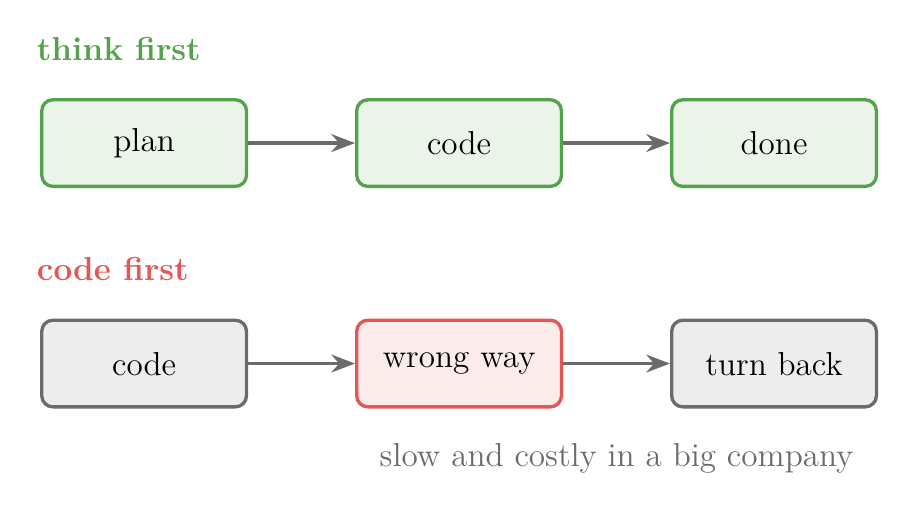
\begin{tikzpicture}[every node/.append style={font=\sffamily\large}]
\tikzset{note/.style={font=\sffamily\large, text=cgrey, align=center}}
  \node[font=\sffamily\bfseries\large, text=cgreen, anchor=west] at (-1.5,1.2) {think first};
  \node[box=cgreen, minimum width=2.6cm] (p) at (0,0) {plan};
  \node[box=cgreen, minimum width=2.6cm] (c) at (4,0) {code};
  \node[box=cgreen, minimum width=2.6cm] (d) at (8,0) {done};
  \draw[arrow] (p) -- (c); \draw[arrow] (c) -- (d);
  \node[font=\sffamily\bfseries\large, text=cred, anchor=west] at (-1.5,-1.6) {code first};
  \node[box=cgrey, minimum width=2.6cm] (c2) at (0,-2.8) {code};
  \node[box=cred, minimum width=2.6cm] (w) at (4,-2.8) {wrong way};
  \node[box=cgrey, minimum width=2.6cm] (t) at (8,-2.8) {turn back};
  \draw[arrow] (c2) -- (w); \draw[arrow] (w) -- (t);
  \node[note] at (6,-4.0) {slow and costly in a big company};
\end{tikzpicture}
\end{document}
